\documentclass{paper}

%\usepackage{times}
\usepackage{epsfig}
\usepackage{graphicx}
\usepackage{amsmath}
\usepackage{amssymb}
\usepackage{color}
\usepackage{caption}
\usepackage{subcaption}


% load package with ``framed'' and ``numbered'' option.
%\usepackage[framed,numbered,autolinebreaks,useliterate]{mcode}

% something NOT relevant to the usage of the package.
\setlength{\parindent}{0pt}
\setlength{\parskip}{18pt}
\graphicspath{{images/}}


\usepackage[latin1]{inputenc}
\usepackage[T1]{fontenc}


\usepackage{listings}
\lstset{%
   language=R,
   basicstyle=\small\ttfamily,
   frame=single
}



\title{Assignment 7}



\author{Jenni Simon\\09-116-005}
% //////////////////////////////////////////////////


\begin{document}



\maketitle


% Add figures:
%\begin{figure}[t]
%%\begin{center}
%\quad\quad   \includegraphics[width=1\linewidth]{ass2}
%%\end{center}
%
%\label{fig:performance}
%\end{figure}


\paragraph{Exercise 1}

\subparagraph{a)}

I assumed that the regression models are supposed to be linear, so I chose the single linear regression model $PRP \sim MMAX$ 
as in assignment 4 and the multiple linear regression model $PRP\sim MMAX+CACH+MMIN+CHMAX+MYCT$ as found in 
assignment 5. Figure \ref{fig:smComp} shows the MSR per fold of the 10-fold cross validation. Note that the folds are identical for both models.


\begin{figure}[h]
\begin{center}
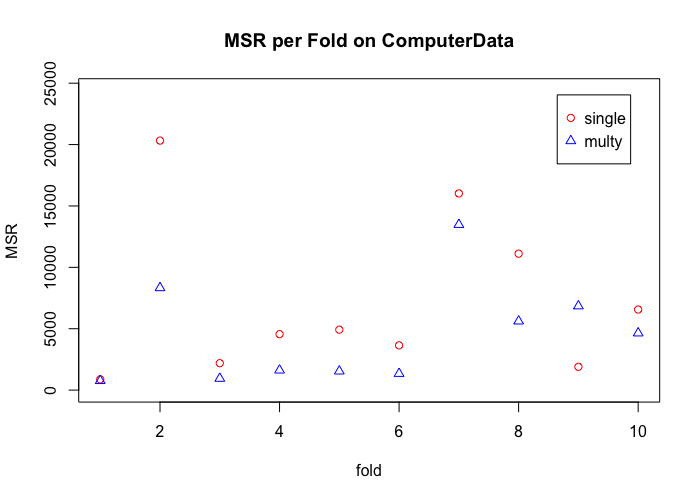
\includegraphics[width=0.8\linewidth]{smComp}
\end{center}
\caption{Mean squared residuals on the ten cross-validation test-sets from the Computer dataset . }
\label{fig:smComp}
\end{figure}

To compare the models the two-sided paired t-test is performed. The results shown in Listing \ref{list:res1} suggest that multiple regression 
performs better given the positive mean difference and relatively low p-value. However, at a significance level of  95\% the Null-hypothesis 
that there is no difference in means can not be rejected.

\begin{minipage}{\linewidth}
  \begin{lstlisting}[caption={Results of paired t-test single vs. multiple regression.},
    label=list:res1]
	Paired t-test

data:  err.single and err.multy
t = 2.0074, df = 9, p-value = 0.07564
alternative hypothesis: difference in means is not equal to 0
95 percent confidence interval:
 -342.6602 5743.2296
sample estimates:
mean of the differences 
               2700.285 
  \end{lstlisting}
\end{minipage}


\subparagraph{b)}

To find the best value for $k$, 10-fold cross-validation has been performed. The resulting average MSR for different $k$'s are shown in 
Figure \ref{fig:knnComp}. A value of $k=1$ clearly gives the best performance in this setting.

\begin{figure}[h]
\begin{center}
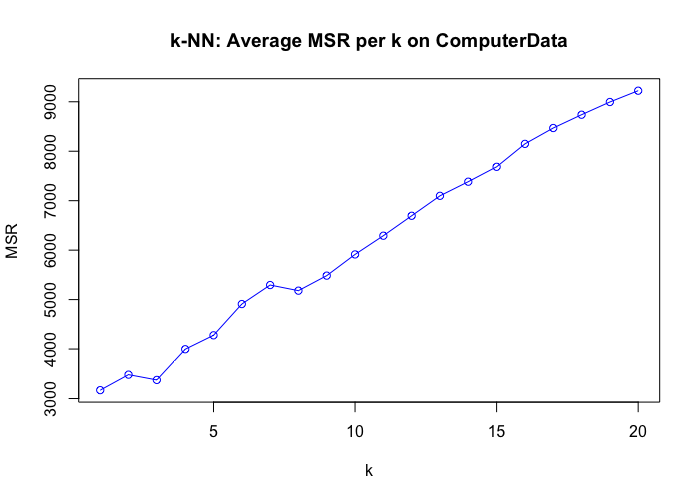
\includegraphics[width=0.8\linewidth]{knnComp}
\end{center}
\caption{Average mean squared residuals on the ten cross-validation test-sets from the Computer dataset  for different values of $k$. }
\label{fig:knnComp}
\end{figure}


\subparagraph{c)}

Figure \ref{fig:vsComp} compares the MSR for 1-NN and the multiple regression model $PRP\sim MMAX+CACH+MMIN+CHMAX+MYCT$
on identical cross-validation folds. 

\begin{figure}[h]
\begin{center}
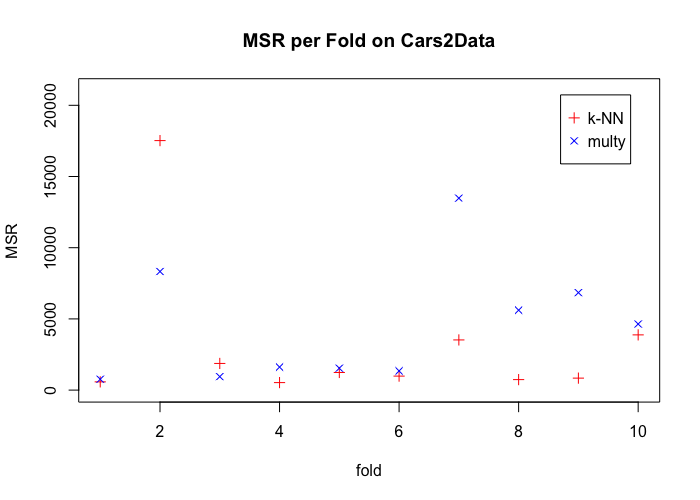
\includegraphics[width=0.8\linewidth]{vsComp}
\end{center}
\caption{Mean squared residuals on the ten cross-validation test-sets from the Computer dataset.  }
\label{fig:vsComp}
\end{figure}

The results of the two-sided paired t-test are shown in Listing \ref{list:res2}. Given the high p-value the Null-hypothesis can not be rejected 
and we can not asses that one model performs better than the other. 

In this case I would favour the multiple linear regression model for its simplicity and better interpretability. Linear models also generalise better
 with little training data and have a much lower bias. 

\begin{minipage}{\linewidth}
  \begin{lstlisting}[caption={Results of paired t-test 1-NN vs. multiple regression.},
    label=list:res2]
Paired t-test

data:  err.knn and err.multy
t = -0.8421, df = 9, p-value = 0.4215
alternative hypothesis: difference in means is not equal to 0
95 percent confidence interval:
 -4944.528  2261.889
sample estimates:
mean of the differences 
               -1341.32 
  \end{lstlisting}
\end{minipage}



\paragraph{Exercise 2}


\subparagraph{a)}

I chose the single linear regression model $mpg \sim weight$ as in assignment 4 and the multiple linear regression model $mpg\sim weight+year$ as found in 
assignment 5. Figure \ref{fig:smCars} shows the MSR per fold of the 10-fold cross validation.

\begin{figure}[h]
\begin{center}
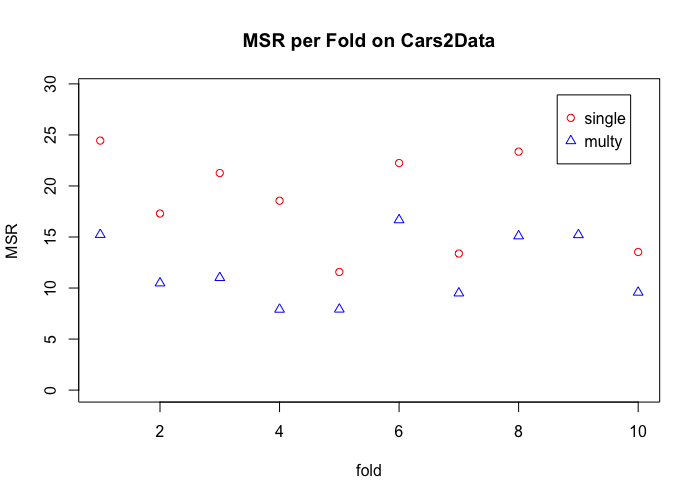
\includegraphics[width=0.8\linewidth]{smCars}
\end{center}
\caption{Mean squared residuals on the ten cross-validation test-sets from the Cars dataset . }
\label{fig:smCars}
\end{figure}

To compare the models the two-sided paired t-test is performed. The results shown in Listing \ref{list:res3} suggest that multiple regression 
performs significantly better given the very low p-value. 

\begin{minipage}{\linewidth}
  \begin{lstlisting}[caption={Results of paired t-test single vs. multiple regression.},
    label=list:res3]
	Paired t-test

data:  err.single and err.multy
t = 8.3581, df = 9, p-value = 1.558e-05
alternative hypothesis: difference in means is not equal to 0
95 percent confidence interval:
 5.134794 8.945783
sample estimates:
mean of the differences 
               7.040289 
  \end{lstlisting}
\end{minipage}



\subparagraph{b)}

To find the best value for $k$, 10-fold cross-validation has been performed. The resulting average MSR for different $k$'s are shown in 
Figure \ref{fig:knnCars}. A value of $k=2$ clearly gives the best performance in this setting.

\begin{figure}[h]
\begin{center}
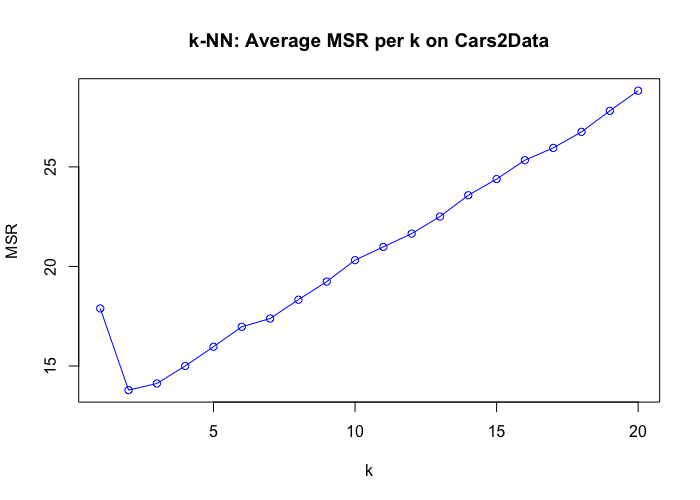
\includegraphics[width=0.8\linewidth]{knnCars}
\end{center}
\caption{Average mean squared residuals on the ten cross-validation test-sets from the Cars dataset  for different values of $k$. }
\label{fig:knnCars}
\end{figure}


\subparagraph{c)}

Figure \ref{fig:vsCars} compares the MSR for 2-NN and the multiple regression model $mpg\sim weight+year$ 
on identical cross-validation folds. 

\begin{figure}[h]
\begin{center}
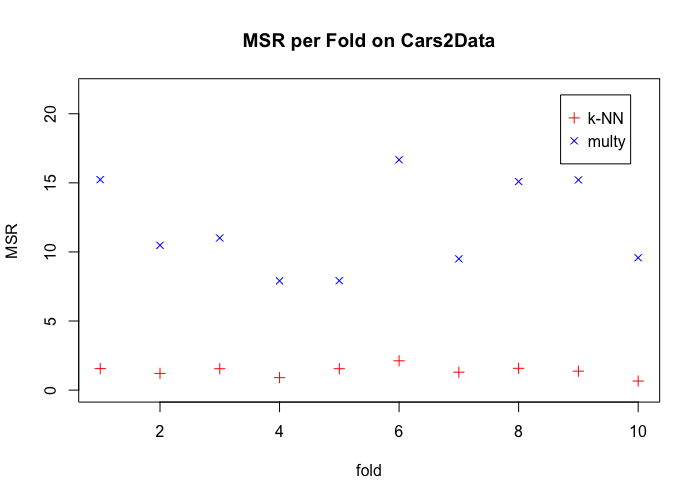
\includegraphics[width=0.8\linewidth]{vsCars}
\end{center}
\caption{Mean squared residuals on the ten cross-validation test-sets from the Cars dataset.  }
\label{fig:vsCars}
\end{figure}

The results of the two-sided paired t-test are shown in Listing \ref{list:res4}. Given the small p-value I would favour the 2-NN model in this case.

\begin{minipage}{\linewidth}
  \begin{lstlisting}[caption={Results of paired t-test 1-NN vs. multiple regression.},
    label=list:res4]
	Paired t-test

data:  err.knn and err.multy
t = 1.9265, df = 9, p-value = 0.08616
alternative hypothesis: difference in means is not equal to 0
95 percent confidence interval:
 -550.3705 6867.0413
sample estimates:
mean of the differences 
               3158.335 
  \end{lstlisting}
\end{minipage}




\end{document}
